Using the emails datasets, there are 1906 number of people who have received emails from Hillary. We selected 10 receivers who have received highest numbers of emails from Clinton directly.
A simple word cloud for all 10 documents can be seen in Figure. \ref{fig:wcloud}
\begin{figure}[h!]
    \centering
    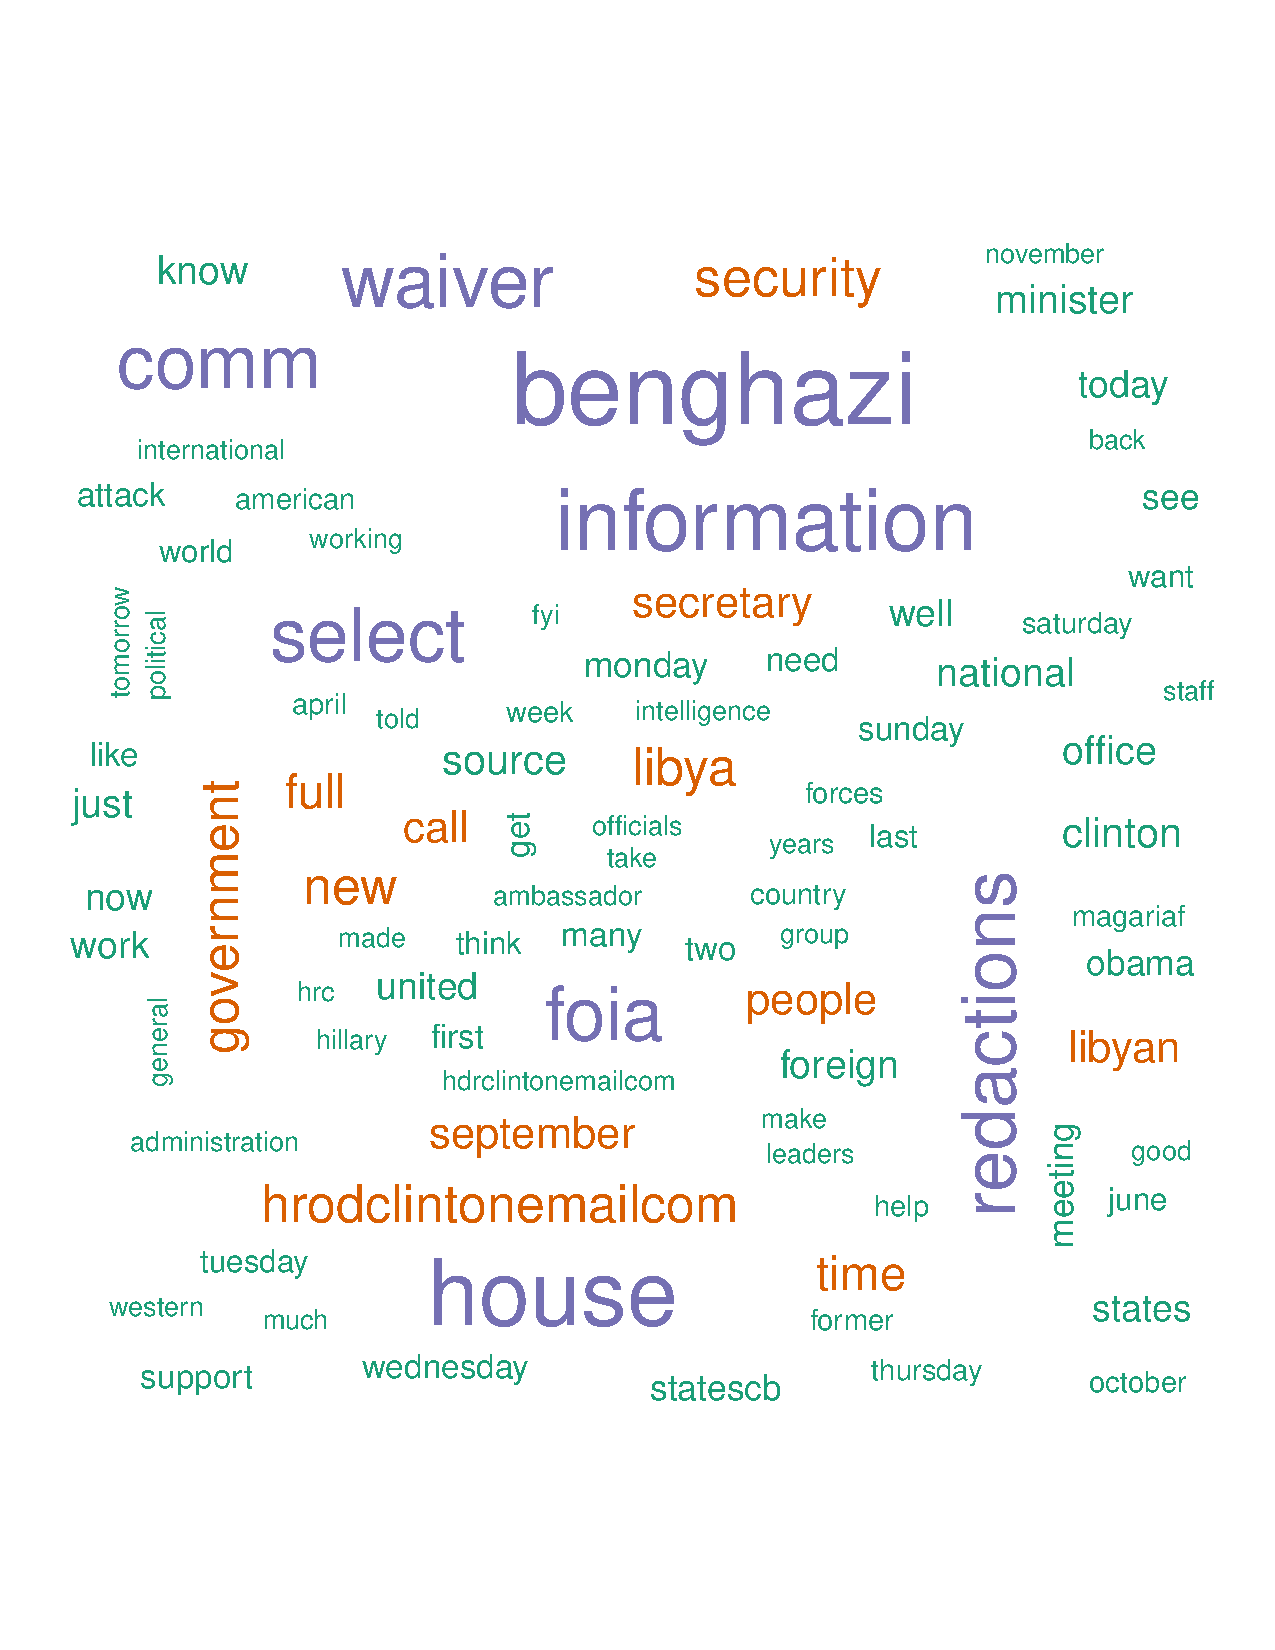
\includegraphics[width=10cm,height=10cm]
    {daitong_and_yihe/wcloud}
    \caption{Word Cloud of Emails}
    \label{fig:wcloud}
\end{figure}

\newpage
\subsection*{Clustering Results}
After obtaining the matrix containing the distances between each documents, we tried two methods: hierarchical clustering and K-means. 
\\
For hierarchical clustering, we have used ward.D method or the Ward's minimum variance method. Figure \ref{fig:dendr} is a cluster dendrogram of the top 10 email accounts. The different colours represents the grouping. The height represents the distance between each document. For example, at distance of 800 we can separate the group in pink and others. The calculation of distance is explained in the section above.
\begin{figure}[h!]
    \centering
    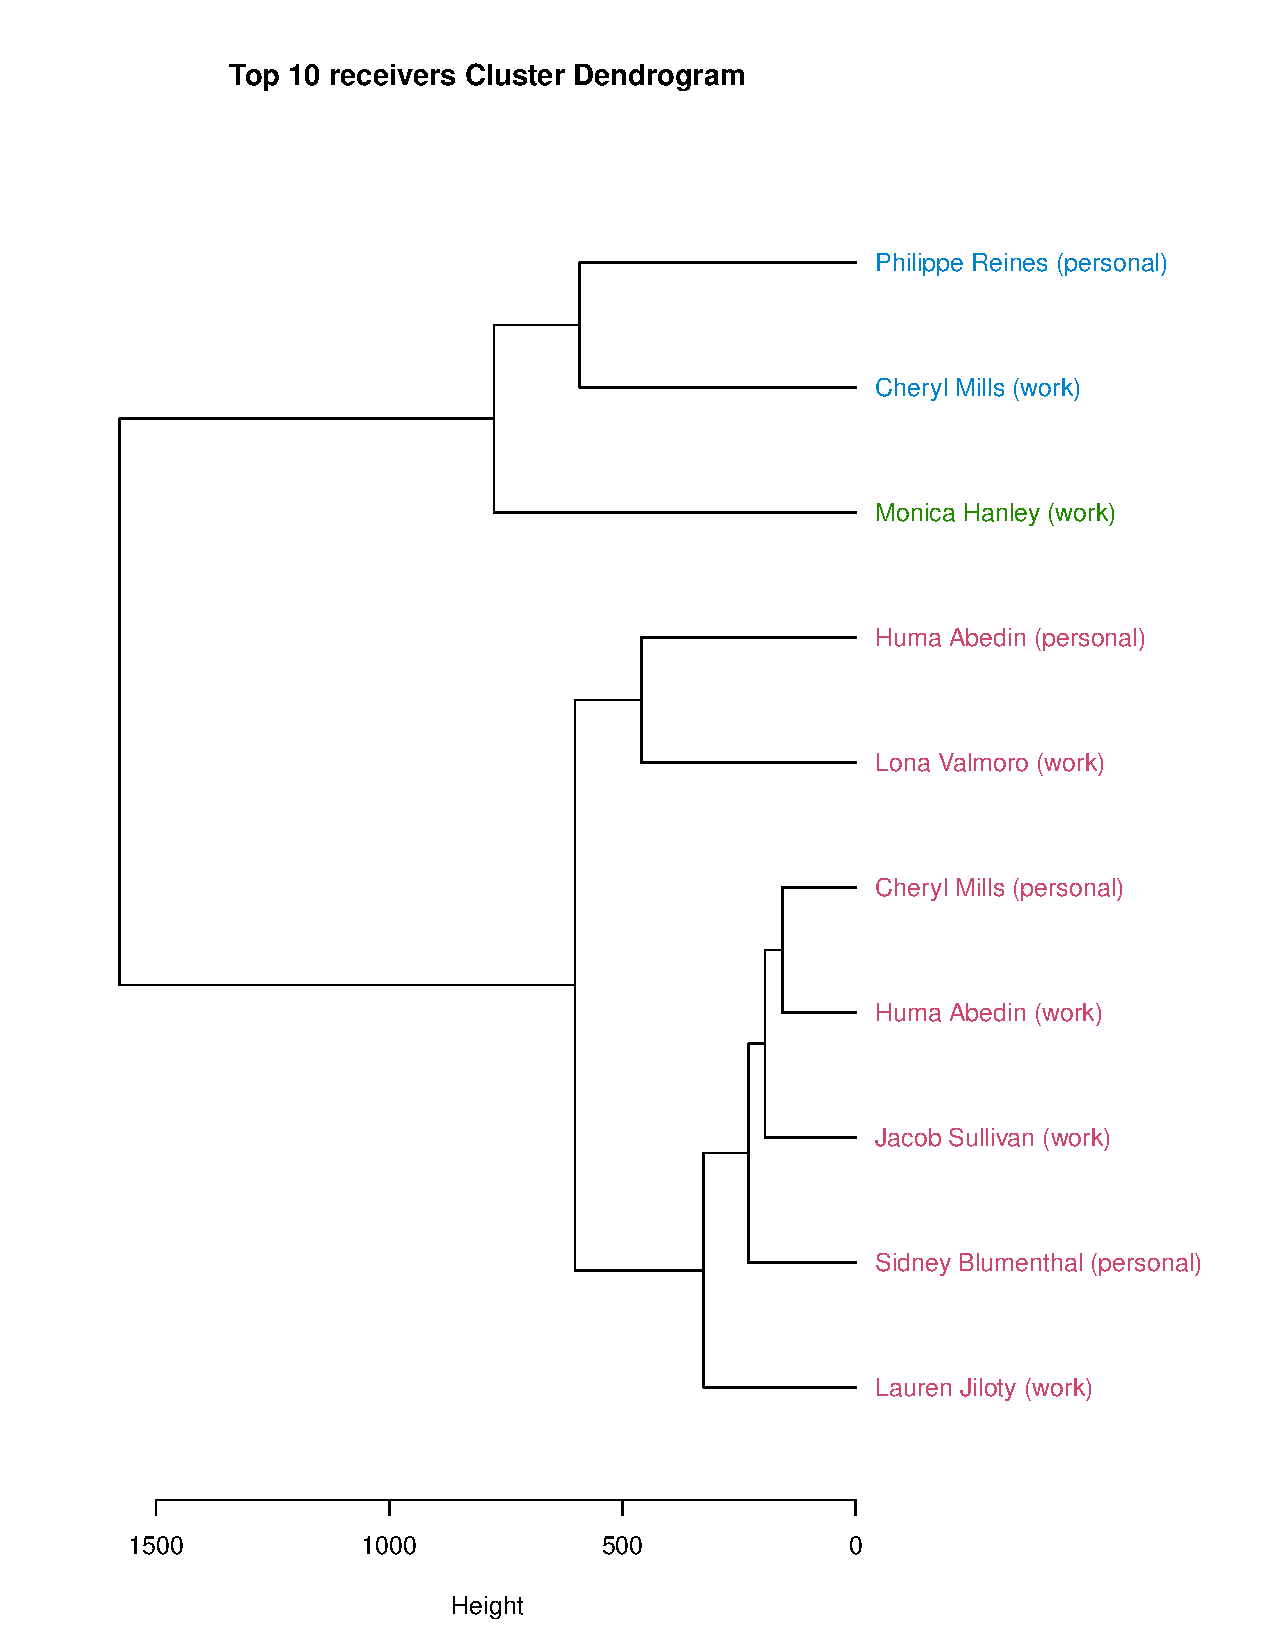
\includegraphics[width=10cm,height=10cm]
    {daitong_and_yihe/clusterp}
    \caption{Dendrogram of top 10 receiver accounts}
    \label{fig:dendr}
\end{figure}

We can also use K-means to determine the clusters. By plotting the within group sum of square errors versus K, we can see from Figure \ref{fig:determine} that K=2 or K=3 might be appropriete group numbers for this dataset.
\begin{figure}[h!]
    \centering
    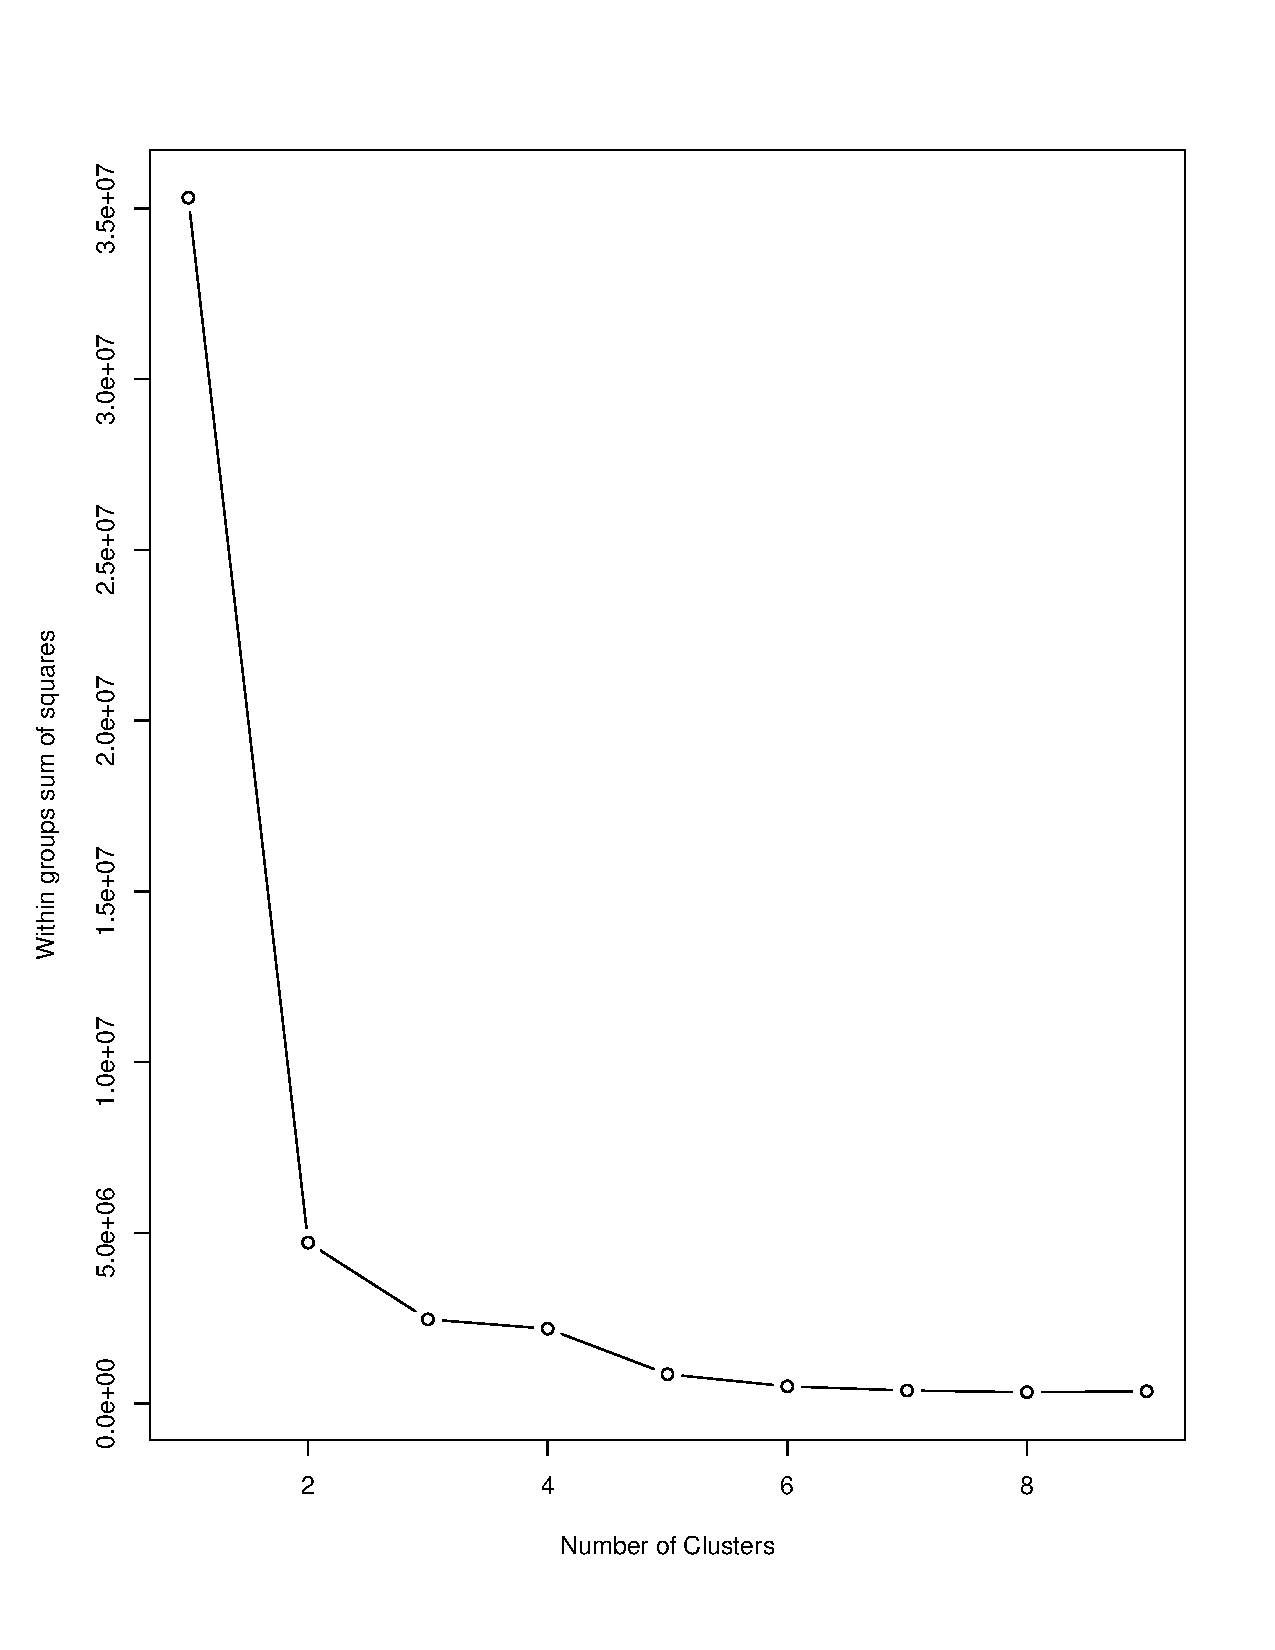
\includegraphics[width=10cm,height=10cm]
    {daitong_and_yihe/clusterd}
    \caption{Within group sum of square errors versus K=1,...,9}
    \label{fig:determine}
\end{figure}


The cluster plots with K=2 and K=3 can be shown in Figure 3 and 4 below. The x and y axis are represented by the first and second component from the PCA analysis. As we can see that the first two components explain more than 95\% of the variance, allowing the clusters to be well separated. 
\\
The results of K-means agree with the results from hierachical clustering. With K=2, we have Sidney Blumenthal (personal), Cheryl Mills (personal) and Monica Hanley (work) in one group (call it Cluster 1) and other accounts in the second group. With K=3, we have Sidney Blumenthal (personal), Cheryl Mills (personal) in group one, Monica Hanley (work) in group two and other accounts in group 3. The clusters can be seen in Figure.\ref{fig:c2} and \ref{fig:c3}.

\begin{figure}[h!]
    \centering
    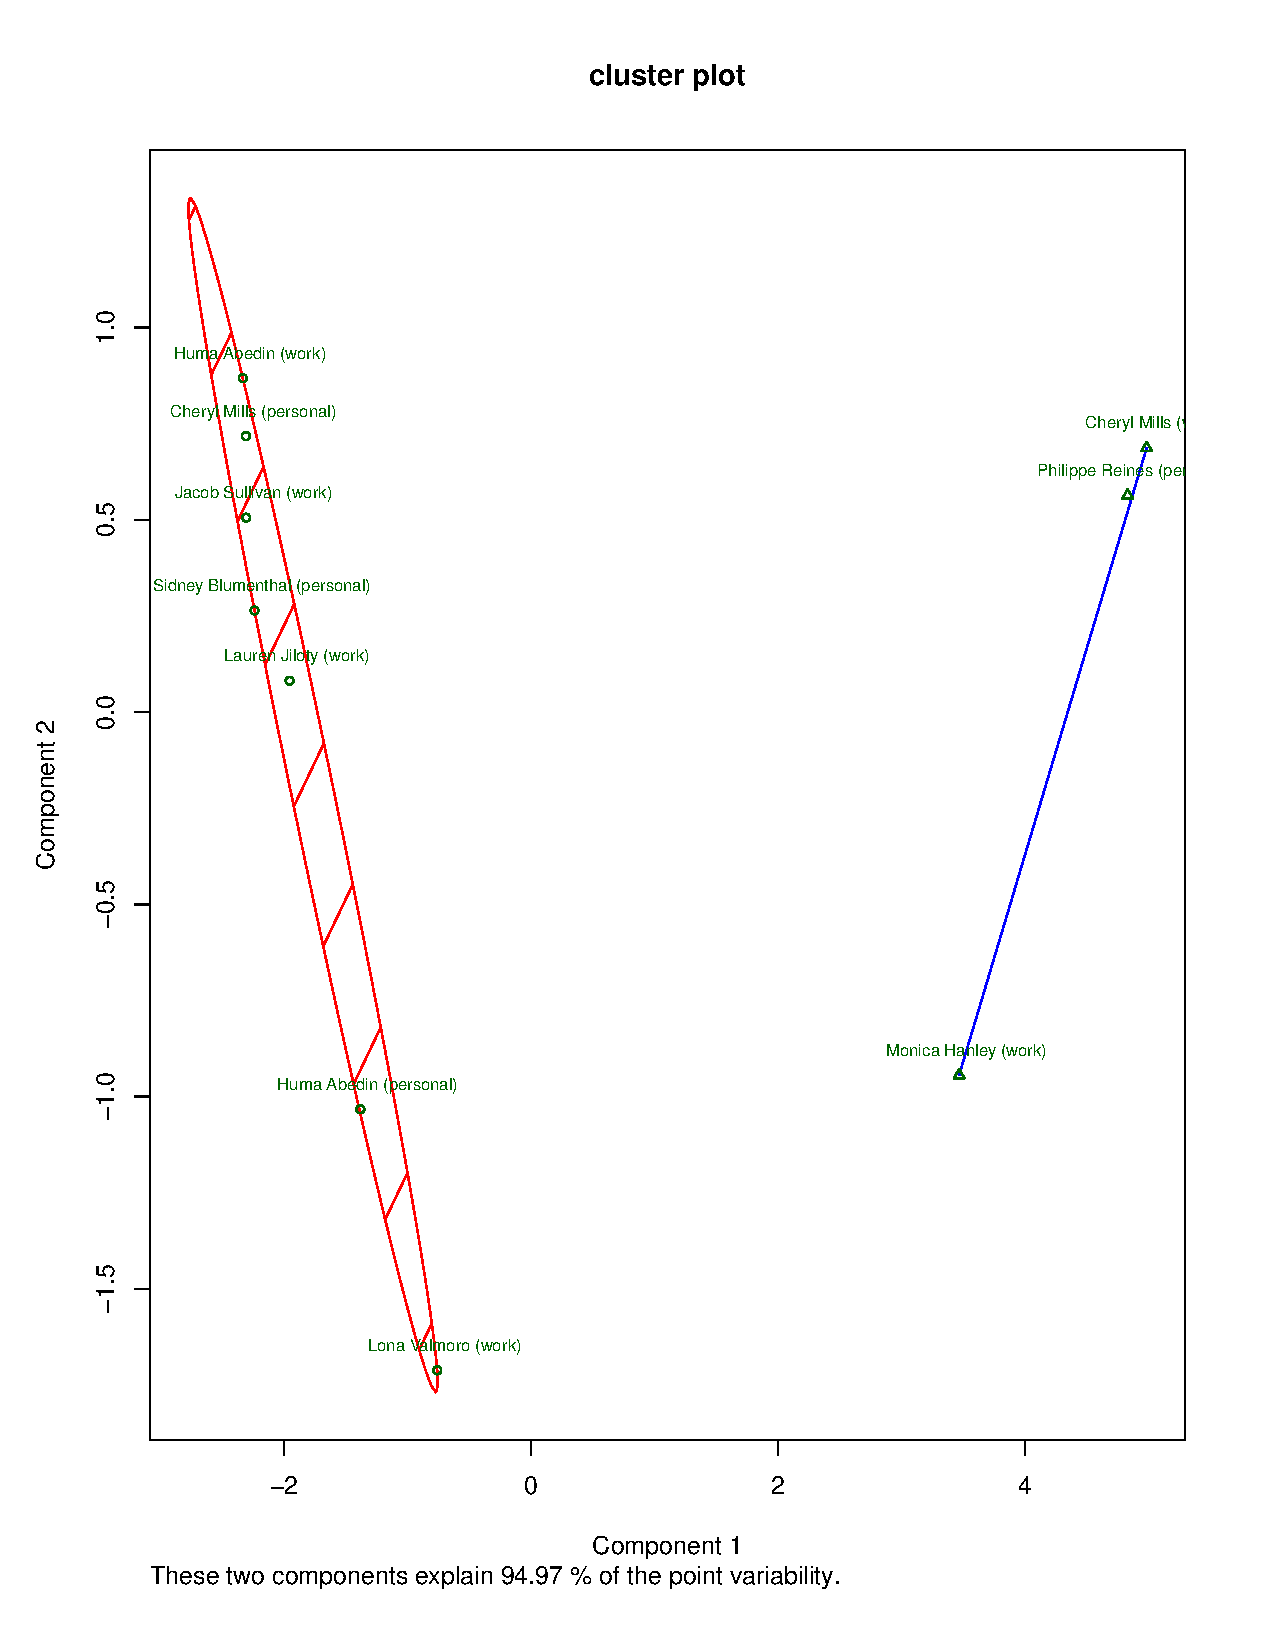
\includegraphics[width=10cm,height=9cm]
    {daitong_and_yihe/c2}
    \caption{Cluster Plot with K=2}
    \label{fig:c2}
\end{figure}

\begin{figure}[h!]
    \centering
    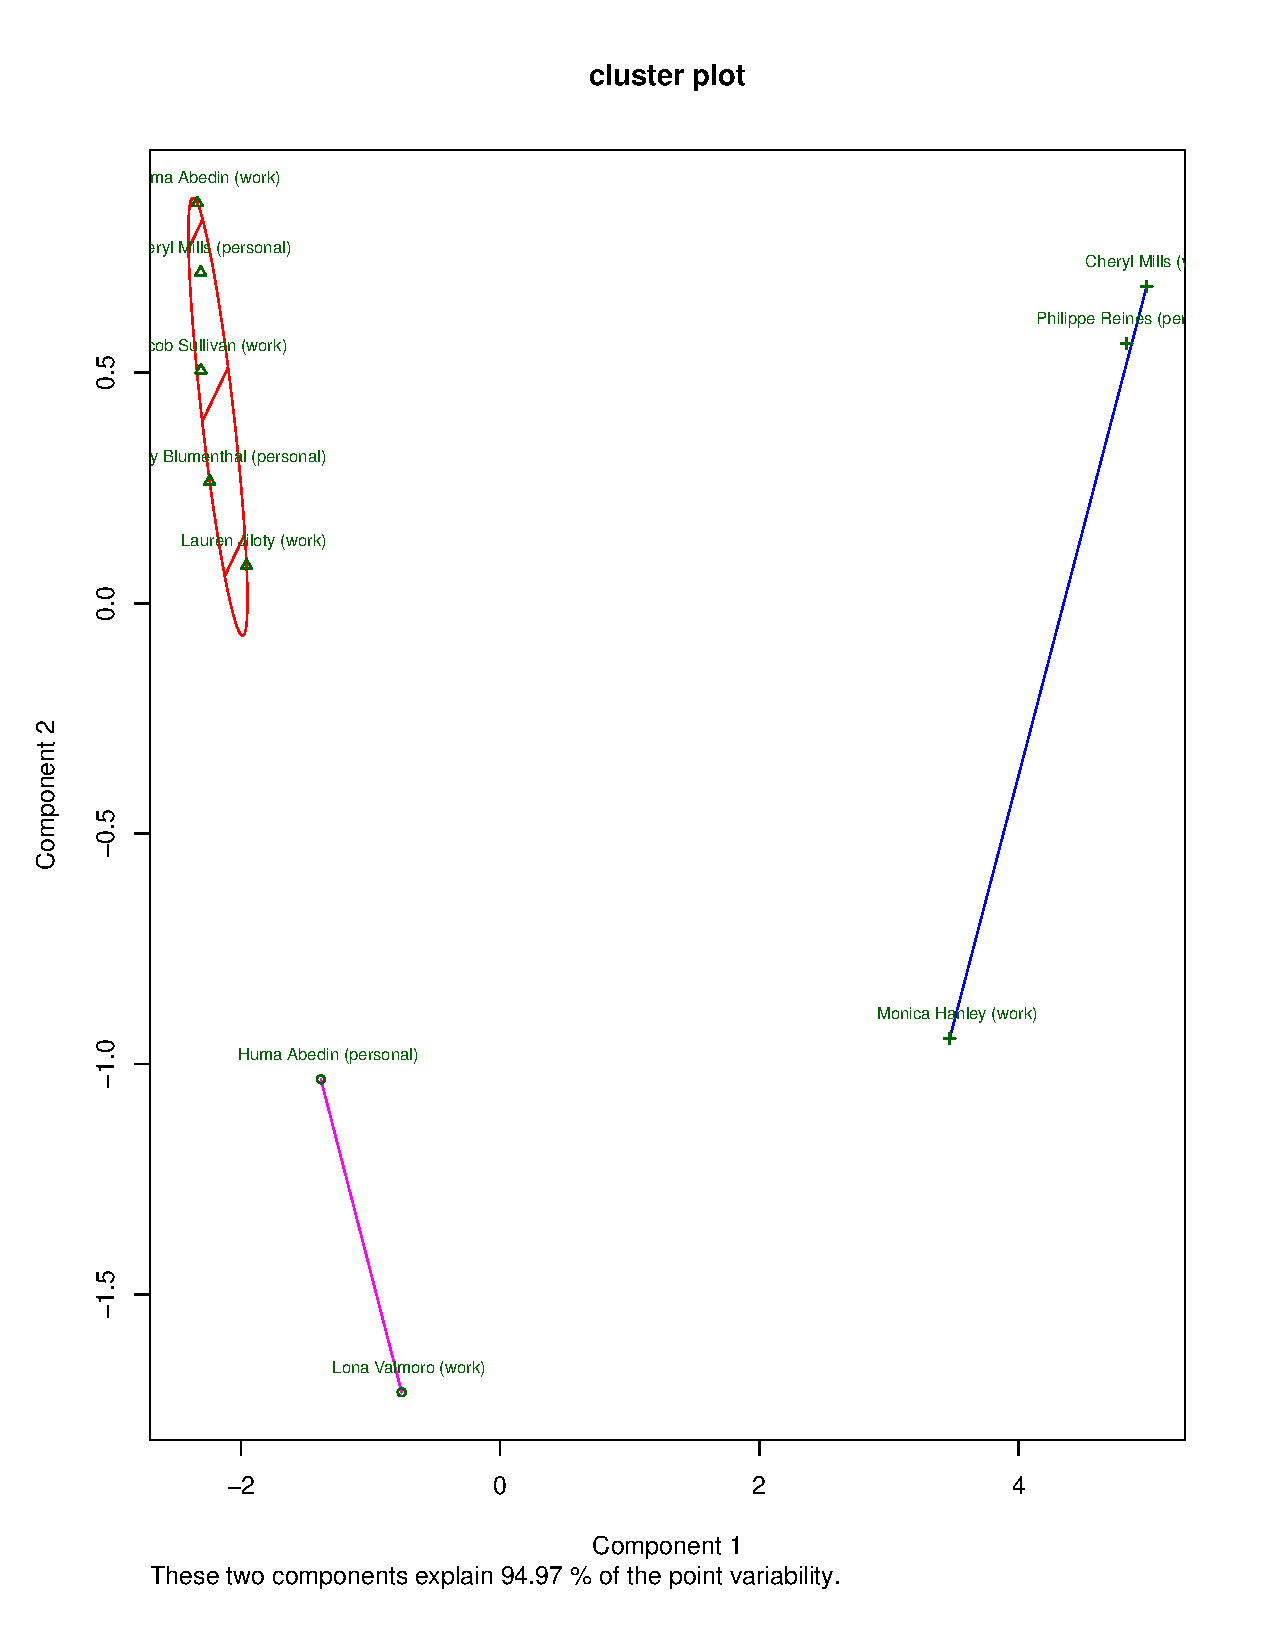
\includegraphics[width=10cm,height=9cm]
    {daitong_and_yihe/c3}
    \caption{Cluster Plot with K=3}
    \label{fig:c2}
\end{figure}

\newpage
Further more, we can inspect the most frequent words mentioned by Clinton to each cluster of receivers. Below is the top 5 words used by each of the two clusters. Both clusters share common words like Benghazi, sensitive and house; though Hillary talked about the term 'agreement' more with the journalist and the lawyer; and the term 'release' more with her aides and advisors. 
\\

\begin{center}
\begin{tabular}{ |p{3cm}|p{3cm}|| p{3cm}|p{3cm}|  }
 \hline
 \multicolumn{4}{|c|}{Top 5 Most Frequent Words} \\
 \hline
 Words (Cluster 1)  & Percentage of Occurance & Words (Cluster 2) & Percentage of Occurance\\
 \hline
 benghazi & 0.76\% & release  & 0.701\% \\
 house &  0.68\% & benghazi & 0.56\% \\
 sensitive & 0.65\% & house & 0.53\%\\
 information & 0.63\% & information & 0.47\%\\
 agreement & 0.57\% &  sensitive  & 0.46\% \\
 \hline
\end{tabular}
\end{center}
